\documentclass[a4paper, 12pt]{article}
\usepackage{graphicx}
\usepackage{enumitem}
\usepackage{mathtools}
\usepackage{hyperref}
\usepackage{caption}
\usepackage{subcaption}
\def\code#1{\texttt{#1}}
\def\f#1{Figure \ref{fig:#1}}
\begin{document}

\title{\vspace{4.0cm}Reflections and Experiences with OpenCL\\
\large KTH DD2360 HT20}
\author{Pontus Asp}
\date{\today}
\maketitle
\thispagestyle{empty}
\pagenumbering{roman}
\newpage

\clearpage
\pagenumbering{arabic}

% Write here ->

% For this final exercise, kindly write a summary (max 1 A4 page) of your reflections and experiences with OpenCL, particularly when contrasting them against CUDA. Include atleast the following two discussion points:
%
%   * Reflect on the useability and easy-of-use of OpenCL contra Nvidia CUDA
%
%   * Contrast the performance of OpenCL contra Nvidia CUDA. Was the performance of your written the same, or did you find any anomalies? If you did find any anomalies, what could have caused these?
%
\section{Thoughts on OpenCL compared to CUDA}
When getting started with OpenCL it is easy to be overwhelmed by the amount of boilerplate code that needs to be written, and what function calls are needed for the setup etc. It is simply a steep learning curve to learn about for instance what contexts and command queues are, or about what the differences between devices and platforms, programs and kernels are. However the fact that OpenCL is so general and works on so many platforms is a very strong argument to using it. CUDA on the other hand, only works on Nvidia GPUs, and this could be both a good, and a bad thing. In my opinion, CUDA is much easier to get into, with less to remember than OpenCL, and with less boilerplate code. CUDA is also made specifically for GPUs, which is what makes it able to be a bit more simple than OpenCL since it has to take less platforms into account. With all this in mind, I do prefer using CUDA, but will probably use OpenCL since it works on more platforms.

Another thing to also consider is the performance differences between CUDA and OpenCL. Of course, CUDA should be faster on a Nvidia GPU since it is Nvidia's own API to their drivers but the question is - in reality, does it make a difference? I tested this by running the two particle simulations we created since I made them both equivalent on the CUDA and OpenCL implementation. My results actually surprised me. The OpenCL performed better than my CUDA variant when using more iterations and particles. But on fewer elements and iterations my CUDA implementation took the lead. I think the CUDA variant however has more room for optimization and if done properly could beat OpenCL at the higher amounts of particles and iterations. 

% Write here <--

\end{document}



%\begin{figure}
%  \centering
%  \begin{subfigure}{.5\textwidth}
%    \centering
%    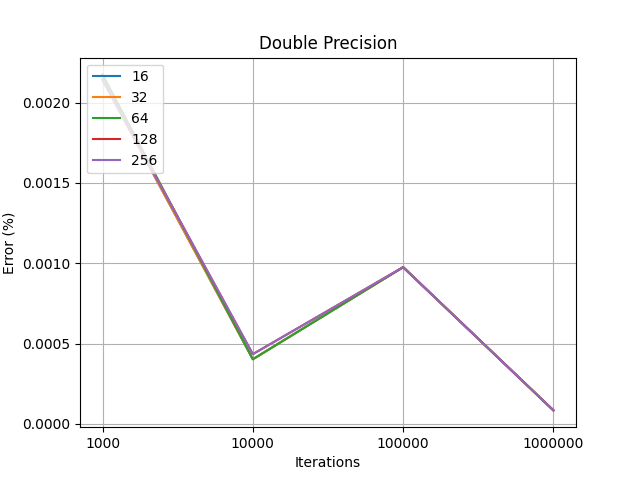
\includegraphics[width=1\linewidth]{graphs/ex_bonus_double_error.png}
%    \caption{Double Precision}
%    \label{fig:ex-single-double-error}
%  \end{subfigure}%
%  \begin{subfigure}{.5\textwidth}
%    \centering
%    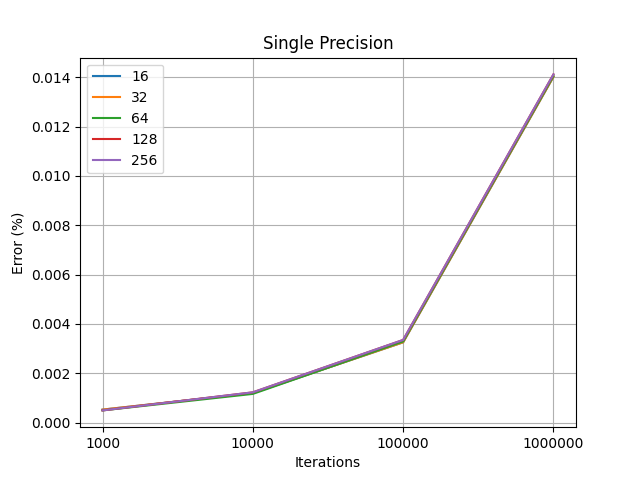
\includegraphics[width=1\linewidth]{graphs/ex_bonus_single_error.png}
%    \caption{Single Precision}
%    \label{fig:ex-bonus-single-error}
%  \end{subfigure}
%  \caption{Graphs of error using double and single precision with different amounts of iterations and block sizes.}
%  \label{fig:fig:ex-bonus-error}
%\end{figure}